\documentclass[journal,12pt,twocolumn]{IEEEtran}
\usepackage{setspace}
\usepackage{gensymb}
\usepackage{xcolor}
\usepackage{caption}
\singlespacing
\usepackage{siunitx}
\usepackage[cmex10]{amsmath}
\usepackage{mathtools}
\usepackage{hyperref}
\usepackage{amsthm}
\usepackage{mathrsfs}
\usepackage{txfonts}
\usepackage{stfloats}
\usepackage{cite}
\usepackage{cases}
\usepackage{subfig}
\usepackage{longtable}
\usepackage{multirow}
\usepackage{enumitem}
\usepackage{bm}
\usepackage{mathtools}
\usepackage{listings}
\usepackage{tikz}
\usetikzlibrary{shapes,arrows,positioning}
\usepackage{circuitikz}
\renewcommand{\vec}[1]{\boldsymbol{\mathbf{#1}}}
\DeclareMathOperator*{\Res}{Res}
\renewcommand\thesection{\arabic{section}}
\renewcommand\thesubsection{\thesection.\arabic{subsection}}
\renewcommand\thesubsubsection{\thesubsection.\arabic{subsubsection}}

\renewcommand\thesectiondis{\arabic{section}}
\renewcommand\thesubsectiondis{\thesectiondis.\arabic{subsection}}
\renewcommand\thesubsubsectiondis{\thesubsectiondis.\arabic{subsubsection}}
\hyphenation{op-tical net-works semi-conduc-tor}

\lstset{
language=Python,
frame=single, 
breaklines=true,
columns=fullflexible
}
\begin{document}
\theoremstyle{definition}
\newtheorem{theorem}{Theorem}[section]
\newtheorem{problem}{Problem}
\newtheorem{proposition}{Proposition}[section]
\newtheorem{lemma}{Lemma}[section]
\newtheorem{corollary}[theorem]{Corollary}
\newtheorem{example}{Example}[section]
\newtheorem{definition}{Definition}[section]
\newcommand{\BEQA}{\begin{eqnarray}}
        \newcommand{\EEQA}{\end{eqnarray}}
\newcommand{\define}{\stackrel{\triangle}{=}}
\newcommand{\myvec}[1]{\ensuremath{\begin{pmatrix}#1\end{pmatrix}}}
\newcommand{\mydet}[1]{\ensuremath{\begin{vmatrix}#1\end{vmatrix}}}
\bibliographystyle{IEEEtran}
\providecommand{\nCr}[2]{\,^{#1}C_{#2}} % nCr
\providecommand{\nPr}[2]{\,^{#1}P_{#2}} % nPr
\providecommand{\mbf}{\mathbf}
\providecommand{\pr}[1]{\ensuremath{\Pr\left(#1\right)}}
\providecommand{\qfunc}[1]{\ensuremath{Q\left(#1\right)}}
\providecommand{\sbrak}[1]{\ensuremath{{}\left[#1\right]}}
\providecommand{\lsbrak}[1]{\ensuremath{{}\left[#1\right.}}
\providecommand{\rsbrak}[1]{\ensuremath{{}\left.#1\right]}}
\providecommand{\brak}[1]{\ensuremath{\left(#1\right)}}
\providecommand{\lbrak}[1]{\ensuremath{\left(#1\right.}}
\providecommand{\rbrak}[1]{\ensuremath{\left.#1\right)}}
\providecommand{\cbrak}[1]{\ensuremath{\left\{#1\right\}}}
\providecommand{\lcbrak}[1]{\ensuremath{\left\{#1\right.}}
\providecommand{\rcbrak}[1]{\ensuremath{\left.#1\right\}}}
\theoremstyle{remark}
\newtheorem{rem}{Remark}
\newcommand{\sgn}{\mathop{\mathrm{sgn}}}
\newcommand{\rect}{\mathop{\mathrm{rect}}}
\newcommand{\sinc}{\mathop{\mathrm{sinc}}}
\providecommand{\abs}[1]{\left\vert#1\right\vert}
\providecommand{\res}[1]{\Res\displaylimits_{#1}}
\providecommand{\norm}[1]{\lVert#1\rVert}
\providecommand{\mtx}[1]{\mathbf{#1}}
\providecommand{\mean}[1]{E\left[ #1 \right]}
\providecommand{\fourier}{\overset{\mathcal{F}}{ \rightleftharpoons}}
\providecommand{\ztrans}{\overset{\mathcal{Z}}{ \rightleftharpoons}}
\providecommand{\system}[1]{\overset{\mathcal{#1}}{ \longleftrightarrow}}
\newcommand{\solution}{\noindent \textbf{Solution: }}
\providecommand{\dec}[2]{\ensuremath{\overset{#1}{\underset{#2}{\gtrless}}}}
\let\StandardTheFigure\thefigure
\def\putbox#1#2#3{\makebox[0in][l]{\makebox[#1][l]{}\raisebox{\baselineskip}[0in][0in]{\raisebox{#2}[0in][0in]{#3}}}}
\def\rightbox#1{\makebox[0in][r]{#1}}
\def\centbox#1{\makebox[0in]{#1}}
\def\topbox#1{\raisebox{-\baselineskip}[0in][0in]{#1}}
\def\midbox#1{\raisebox{-0.5\baselineskip}[0in][0in]{#1}}

\vspace{3cm}
\title{11.10.3.10}
\author{Lokesh Surana}
\maketitle
\section*{Class 11, Chapter 10, Exercise 3.10}

Q. The line through the points $(h, 3)$ and $(4, 1)$ intersects the line $7{x} - 9{y} - 19 = 0$ at right angle. Find the value of h.

\solution Let the point $\vec{P}$ be the foot of the perpendicular on the line $7{x} - 9{y} - 19 = 0$ from point $\myvec{h\\3}$ (Let's say point $\vec{O}$).
The optimization problem can be expressed as

\begin{align}
    \label{eq:1}
    \min_{\vec{x}} \norm{\vec{x}-\vec{O}}^2\\
    \text{s.t.} \quad \vec{n}^\top\vec{x} = c
\end{align}

where
\begin{align}
    \vec{n} = \myvec{7 \\ -9},\,c = 19
\end{align}

The line equation can be expressed as
\begin{align}
    \label{eq:2}
    \vec{x} = \vec{A}+\lambda\vec{m}
\end{align}
where
\begin{align}
    \vec{m} = \myvec{9            \\ 7},\,
    \vec{A} = \myvec{\frac{19}{7} \\ 0}
\end{align}

Using the parameric form, Substituting \eqref{eq:2} in \eqref{eq:1}, the optimization problem becomes
\begin{align}
    \min_{\lambda} \norm{ \lambda\vec{m} +\brak{\vec{A}-\vec{O}}}^2
\end{align}

\begin{align}
    \begin{split}
        \label{eq:3}
        \ \implies \min_{\lambda}f\brak{\lambda} = \lambda^2\norm{\vec{m}}^2 + \\ 2\lambda\brak{\vec{A}-\vec{O}}^\top\vec{m} + \norm{\vec{A}-\vec{O}}^2 \
    \end{split}
\end{align}

$\because$ the coefficient of $\lambda^2> 0$, \eqref{eq:3} is a convex function.
Thus,
\begin{align}
    f^{\prime\prime}\brak{\lambda}                                            & = 2\norm{\vec{m}}^2             \\
    \because f^{\prime\prime}\brak{\lambda} > 0, f^\prime\brak{\lambda_{min}} & = 0, \text{ for } \lambda_{min}
\end{align}
yielding
\begin{align}
                  & f^\prime\brak{\lambda_{min}} =  2\lambda_{min}\norm{\vec{m}}^2 + 2\brak{\vec{A}-\vec{O}}^\top\vec{m}  = 0 \\
    \label{eq:4}
    \lambda_{min} & = -\frac{\brak{\vec{A}-\vec{O}}^\top\vec{m}}{\norm{\vec{m}}^2}
\end{align}

It is given that the line through the points $\myvec{h \\ 3}$ and $\myvec{4 \\ 1}$ intersects the line $7{x} - 9{y} - 19 = 0$ at right angle. And the point $\myvec{4 \\ 1}$ is on the line $7{x} - 9{y} - 19 = 0$.

From equation \eqref{eq:2}
\begin{align}
    \implies \myvec{4 \\ 1} &= \myvec{\frac{19}{7} \\ 0} + \lambda_{min}\myvec{9 \\ 7} \\
    \implies \lambda_{min} &= \frac{1}{7} 
\end{align}


Substituting the values of $\vec{A}$, $\vec{O}$, $\lambda_{min}$ and $\vec{m}$ in equation \eqref{eq:4}
\begin{align}
    \frac{1}{7} &= -\frac{\brak{\myvec{\frac{19}{7} \\ 0} -\myvec{h \\ 3}}^\top\myvec{9 \\ 7}}{\norm{\myvec{9 \\ 7}^2}}\\
    \implies \frac{130}{7} &= -\frac{171}{7} + 9{h} + 21\\
    \implies h &= \frac{22}{9}
\end{align}

\begin{figure}[!htb]
    \centering
    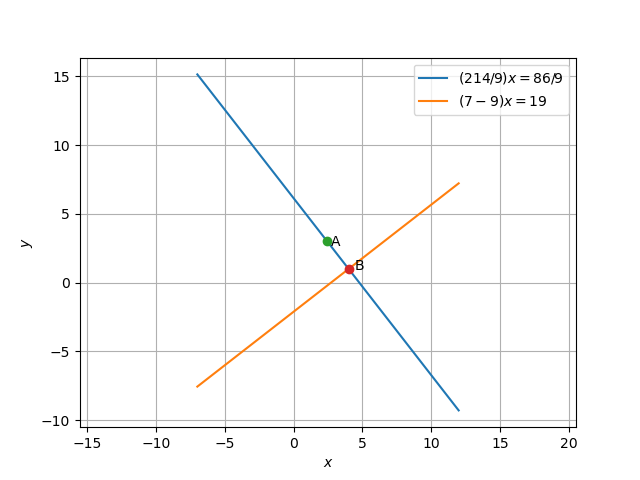
\includegraphics[width=\columnwidth]{figs/lines.png}
    \caption{}
    \label{fig:line}
\end{figure}

\end{document}